%
% -- Manlio Modugno

\documentclass{beamer} 
\usepackage{eulervm}
%\usepackage{booktabs}
\usepackage{listings}
\usepackage{bold-extra}
\usepackage{cancel}
\usepackage{fancybox}
\usepackage{soul}
\usepackage[english]{babel}
\usepackage[utf8]{inputenc}
\usepackage{hyperref}
\usepackage{amsmath}
%\hypersetup{colorlinks=true,urlcolor=blue}

\newcommand{\codefont}{\fontsize{6}{8}\selectfont}
\lstset{language=[Sharp]C, 
captionpos=b, 
frame=lines,
lineskip= 1pt, %space between lines
basicstyle=\codefont, 
keywordstyle=\color{blue}, 
commentstyle=\color{green}, 
stringstyle=\color{red}, 
numbers=left, 
numberstyle=\tiny, 
stepnumber=2,
numbersep=5pt,
breaklines=true, 
breakatwhitespace=false,
showstringspaces=false,
frame=single,
tabsize=2,
emph={double,bool,int,unsigned,char,true,false,void},
emphstyle=\color{blue},
emph={Assert,Test},
emphstyle=\color{red},
emph={[2]\using,\#define,\#ifdef,\#endif},
emphstyle={[2]\color{blue}}
}


\mode<presentation>
\definecolor{title_color}{RGB}{2,128,181} 
\usetheme{Ilmenau}
\usecolortheme[named=title_color]{structure}
\setbeamercolor{palette quaternary}{use=structure,fg=black,bg=white} %header footer color
\useoutertheme[subsection=false]{smoothbars}
\setbeamercovered{transparent}
\setbeamertemplate{navigation symbols}{}
\setbeamerfont{subsection in toc}{size=\scriptsize}

\title{The Dependency Inversion Principle}
\author{Manlio Modugno}
\institute[GMTechnologies] 

\date[]{The Dependency Inversion Principle}

\subject{}

\graphicspath{{img/}}
\pgfdeclareimage[height=0.6cm]{mfg-logo}{img/mfgLogo}
\logo{\pgfuseimage{mfg-logo}}

%
% Content start
%
\begin{document}
\begin{frame}
  \titlepage
\end{frame}

\begin{frame}
  \frametitle{Topics}
  \tableofcontents
\end{frame}


\section{Intro}
\subsection{Intro}
\begin{frame}
  \frametitle{Intro}
  \begin{itemize}
	\item<+-> def A: \textbf{High-level modules should not depend on low-level modules. Both should depend on abstractions}
	\item<+-> def B: \textbf{Abstractions should not depend upon details. Details should depend upon abstractions}
	\item<+-> Why ``inversion''?..
	\item<+-> Because traditional sd approaches create high-level modules that depend on low-level ones and policies that depend upon details.. a good OOD inverts the dependency...
   \end{itemize}
\end{frame}

\begin{frame}
  \frametitle{Intro}
  \begin{itemize}
	\item<+-> High-level modules contain important policy decision and business models.. (i.e. ``identity'' of an application)
	\item<+-> if high-levels depend upon low-levels a change in latter can force modification in high-level
	\item<+-> On the contrary, high-level should influence lower-levels! ...
	\item<+-> We want be able to reuse high-level modules.. but depending upon lowers decrease probability in reuse...  
   \end{itemize}
\end{frame}

\section{Layering}
\subsection{Layering}
\begin{frame}
	\frametitle{Layering}
	``all well structured object-oriented architectures have clearly-defined layers, with each layer providing some coherent set of services through a well-defined and controlled interface''.. pay attention to transitive dependency!
	\begin{center}
	\fbox{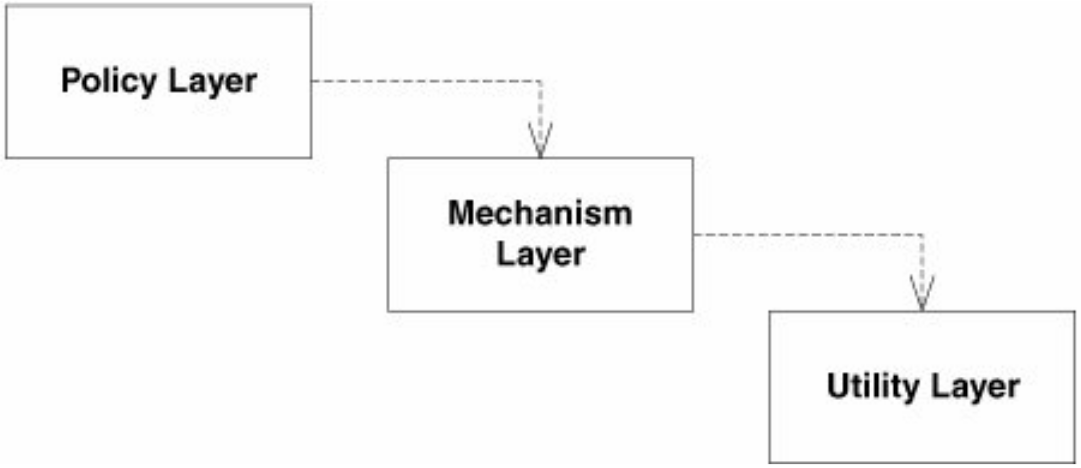
\includegraphics[scale=0.2]{layerBad}}
	\end{center}
\end{frame}

\begin{frame}
	\frametitle{Layering}
	A correct approach is to declare abstract interfaces in upper-levels and let lower interact with them
	\begin{center}
	\fbox{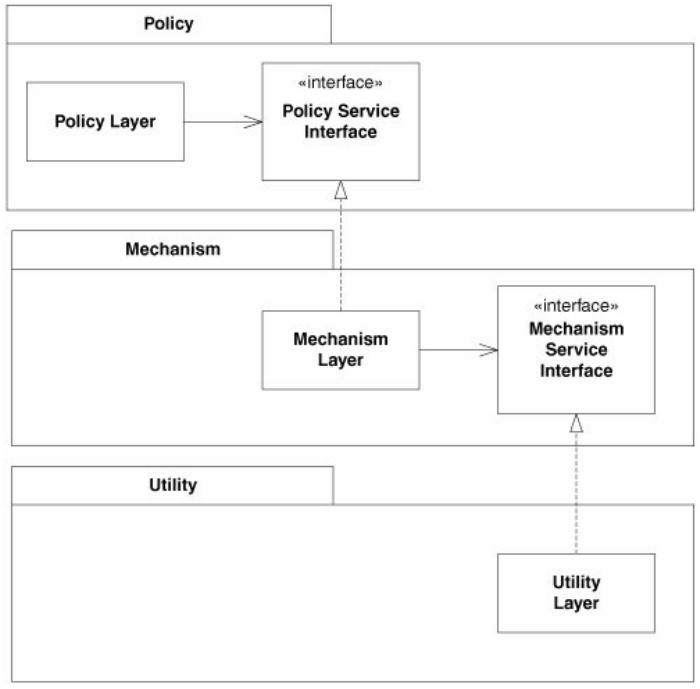
\includegraphics[scale=0.2]{layerGood}}
	\end{center}
\end{frame}

\subsection{Ownership Inversion}
\begin{frame}
  \frametitle{Ownership Inversion}
  \begin{itemize}
	\item<+-> Also interfaces ownership is inverted.. 
	\item<+-> ..clients tend to own the abstract interfaces and that their servers derive from them
	\item<+-> Hollywood principle : ``Don't call us; we'll call you''..
	\item<+-> The lower-level modules provide the implementation for interfaces that are declared within, and called by, the upper-level modules
   \end{itemize}
\end{frame}

\begin{frame}
  \frametitle{Ownership Inversion}
  \begin{itemize}
	\item<+-> Owned interfaces are distributed with the owning clients and not with the servers that implement them
	\item<+-> The interface is in the same package or library with the client. This forces the server library or package to depend on the client library or package
	\item<+-> Always evaluate context.. maybe we don't want server depend on the client..
   \end{itemize}
\end{frame}

\subsection{Dependence on Abstractions}
\begin{frame}
  \frametitle{Dependence on Abstractions}
  \begin{itemize}
	\item<+-> A more general definition could be: ``Depend on abstractions''
	\item<+-> ..that is we shouldn't depend on concrete classes, all relationships should terminate on a abstract class / interface
	\item<+-> No variable should hold a reference to a concrete class. (remember extends is evil?)
	\item<+-> No class should derive from a concrete class.
	\item<+-> No method should override an implemented method of any of its base classes.
  \end{itemize}
\end{frame}

\begin{frame}
  \frametitle{Dependence on Abstractions}
  \begin{itemize}
	\item<+-> Depending on nonvolatile concrete classes should be fine..
	\item<+-> that is, classes that don't change very often (think about String for example..)
	\item<+-> Volatile classes are usually classes that we write..
  \end{itemize}
\end{frame}

\section{A simple DIP example}
\subsection{A simple DIP example}
\begin{frame}
	\frametitle{A simple DIP example}
	DIP can be applied whenever one object sens a message to another. Here \textit{Button} senses in some way the external environment(by switch and so on..) and send accordingly a message to \textit{Lamp}. Physical details are not important..
	\begin{center}
	\fbox{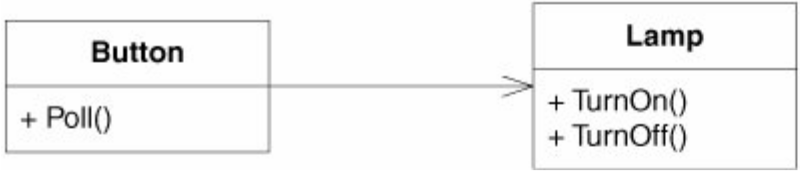
\includegraphics[scale=0.2]{dipExample}}
	\end{center}
\end{frame}

\begin{frame}[containsverbatim]
	\frametitle{A simple DIP example}
	Button depends directly on Lamp. Button will be affected by changes to Lamp and Button can't be reused in other context \\
	\begin{lstlisting}
public class Button{
	private Lamp lamp;
	public void Poll(){
		if (/*some condition*/)
			lamp.TurnOn();
	}
}
	\end{lstlisting}
	This code violates DIP. High-level policies are not separated from lower ones. Button handles only Lamp
\end{frame}


\subsection{Finding the Underlying Abstraction}
\begin{frame}
  \frametitle{Finding the Underlying Abstraction}
  \begin{itemize}
	\item<+-> What is the high-level policy? 
	\item<+-> It is the abstraction that underlies the application, the truths that do not vary when the details are changed
	\item<+-> It is the system inside the system, it is the metaphor
	\item<+-> In the example, the underlying abstraction is to detect an on/off gesture from a user and relay that gesture to a target object
	\item<+->  What mechanism is used to detect the user gesture? Irrelevant! 
	\item<+->  What is the target object? Irrelevant! These are details that do not impact the abstraction
   \end{itemize}
\end{frame}

\begin{frame}
	\frametitle{A simple DIP example}
	Here dependency upon Lamp is inverted by means of ButtonServer,  that can be used to turn on/off something. Lamp now is depending rather that being depended on.
	\begin{center}
	\fbox{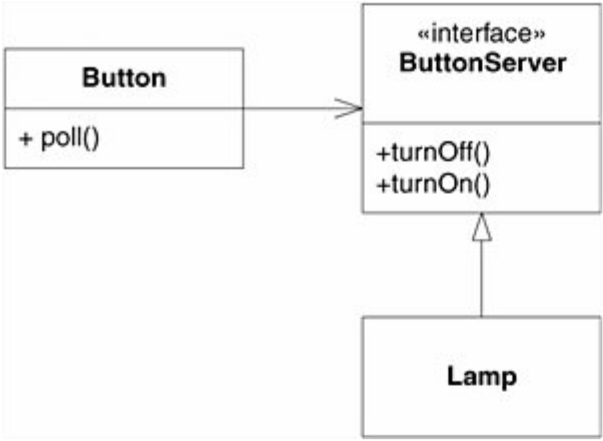
\includegraphics[scale=0.2]{dipExampleGood}}
	\end{center}
\end{frame}

\section{The Furnace example}
\subsection{Furnace Example}
\begin{frame}
  \frametitle{The Furnace example}
  \begin{itemize}
	\item<+-> Consider software controlling a furnace.. 
	\item<+-> Software can read current temperature and instruct furnace to turn on/off
   \end{itemize}
\end{frame}

\begin{frame}[containsverbatim]
	\frametitle{A simple DIP example}
	An example that has a lot of low-level details $ \rightarrow $ can't be reused with different control hardware \\
	\begin{lstlisting}
const byte TERMOMETER = 0x86;
const byte FURNACE = 0x87;
const byte ENGAGE = 1;
const byte DISENGAGE = 0;
void Regulate(double minTemp, double maxTemp) {
	for(;;){
		while (in(THERMOMETER) > minTemp)
			wait(1);
		out(FURNACE,ENGAGE);
		
		while (in(THERMOMETER) < maxTemp)
			wait(1);
		out(FURNACE,DISENGAGE);
	}
}
	\end{lstlisting}
\end{frame}


\begin{frame}
	\frametitle{A generic solution}
	\begin{center}
	\fbox{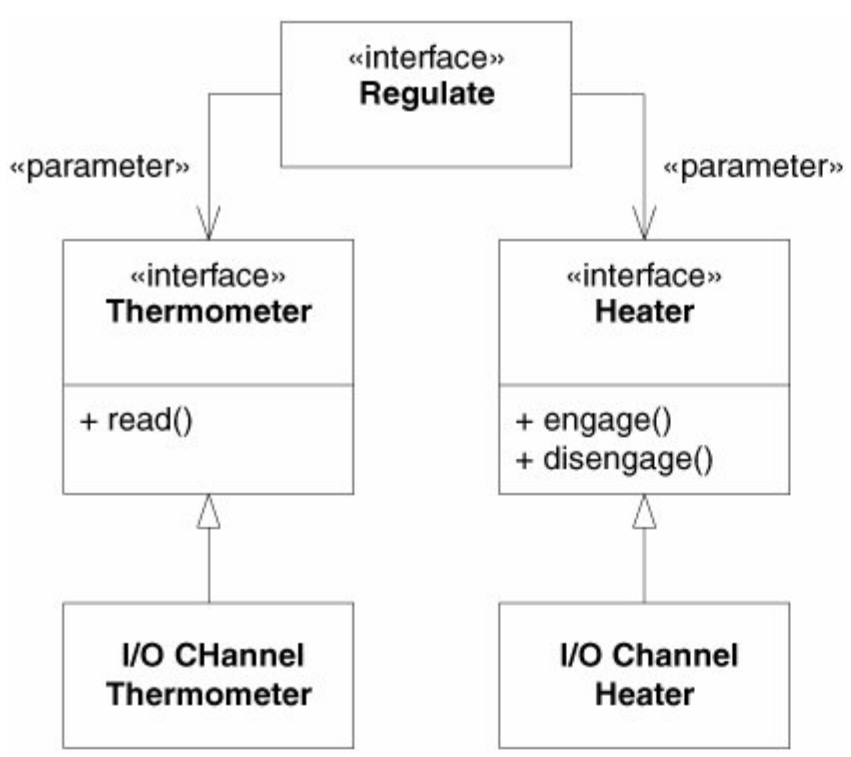
\includegraphics[scale=0.2]{furnace}}
	\end{center}
\end{frame}

\begin{frame}[containsverbatim]
	\frametitle{A simple DIP example}
	Regualate takes two interfaces as arguments. High-level regulation policies now do not depends on any specific details.. \\
	\begin{lstlisting}
void Regulate(Thermometer t, Heater h, double minTemp, double maxTemp){
	for(;;){
		while (t.Read() > minTemp)
			wait(1);
		h.Engage();

		while (t.Read() < maxTemp)
			wait(1);
		h.Disengage();
	}
}
	\end{lstlisting}
\end{frame}

\section{Conclusion}
\subsection{Conclusion}
\begin{frame}
  \frametitle{Conclusion}
  \begin{itemize}
	\item<+-> Programming can creates a dependency structure in which policy depends on detail
	\item<+-> OOP can invert dependency and mitigate problem on change of details..
	\item<+-> Inversion of dependencies is the hallmark of good object-oriented design (i.e. get the metaphor under the metaphor..)
	\item<+->  It doesn't matter what language a program is written in..OO is OO
	\item<+-> DIP is the fundamental low-level mechanism behind many of the benefits claimed for object-oriented technology
	\item<+-> It is critically important for the construction of code that is resilient to change
   \end{itemize}
\end{frame}

\end{document}
